\documentclass[11pt]{article}
\usepackage{amsmath,textcomp,amssymb,geometry,graphicx,rotating,multirow, listings}

\lstset{breaklines=true}

\def\Name{Sahar Mesri, Sagar Karandikar}
\def\Login{cs150-bw, cs150-bn}

\title{CS150 Checkpoint 3 Proposal, Team 07}
\author{\Name, \texttt{\Login}}
\pagestyle{myheadings}

\begin{document}
\maketitle
\section*{1. Block Diagrams}

\subsection*{Overall System}

\noindent\includegraphics[scale=0.15]{modules/overall.png}

\subsection*{a. Gaussian Filter Banks}

Octave Module:

Delay blocks are 2112 byte wide shift registers.

\noindent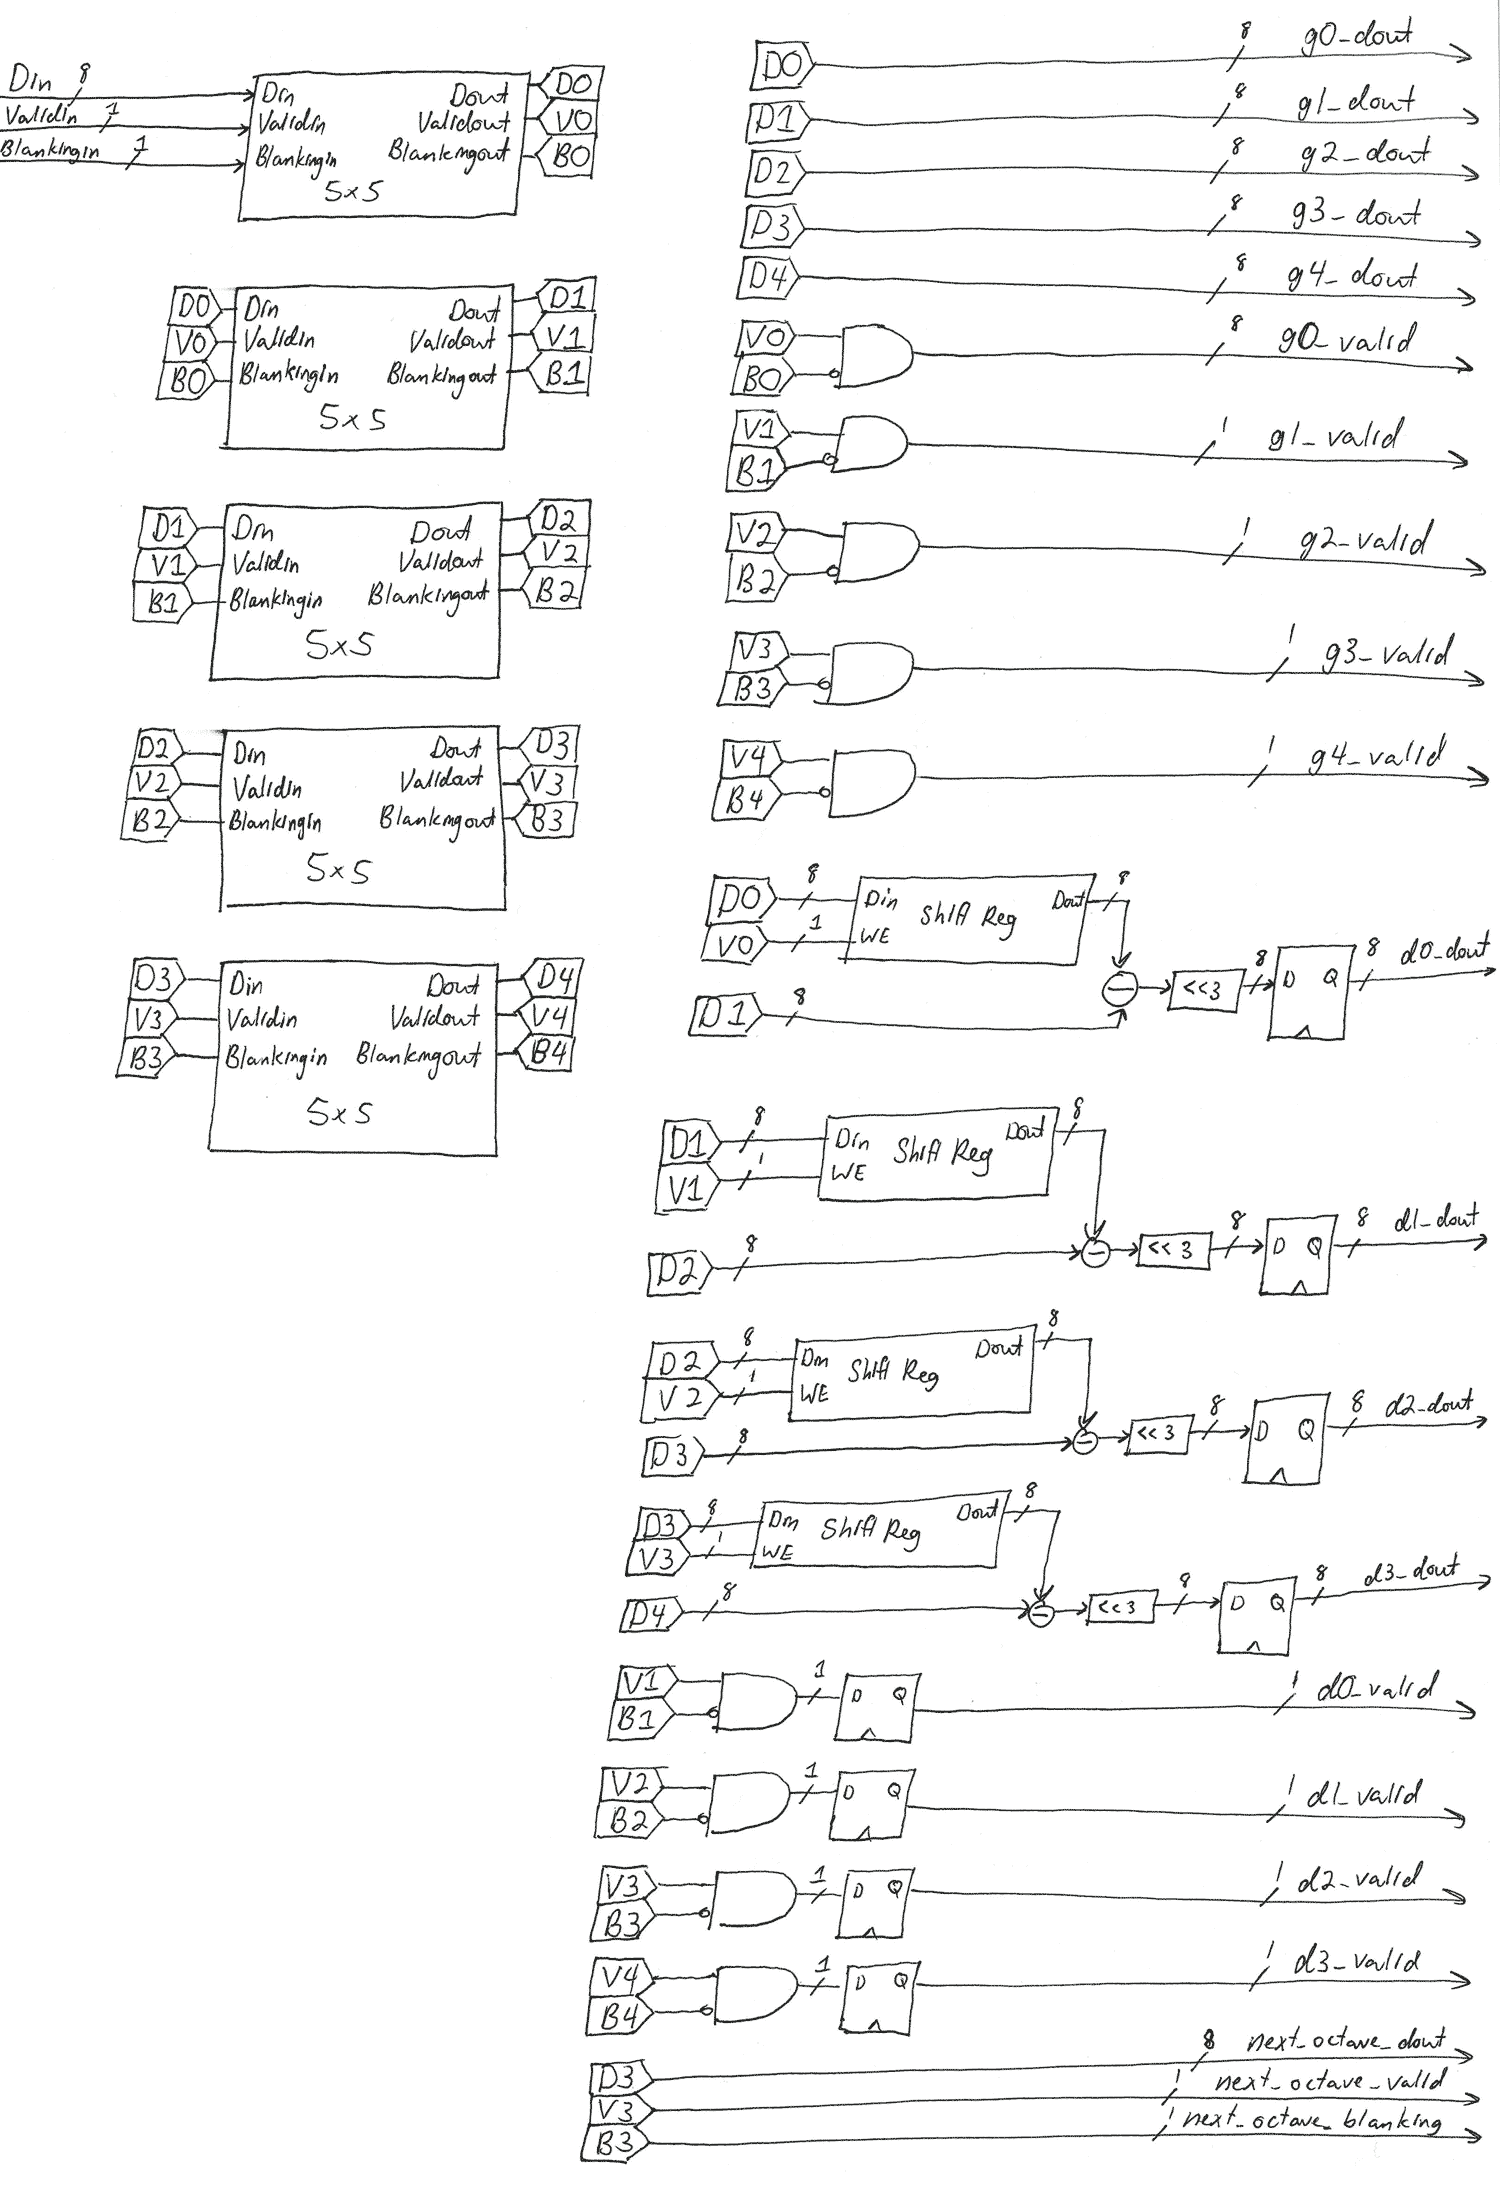
\includegraphics[scale=0.15]{modules/octave.png}

5x5 Window Module:

Delay block is 2112 bit wide shift register.

\noindent\includegraphics[scale=0.15]{modules/5x5window.png}

X Window Module:

\noindent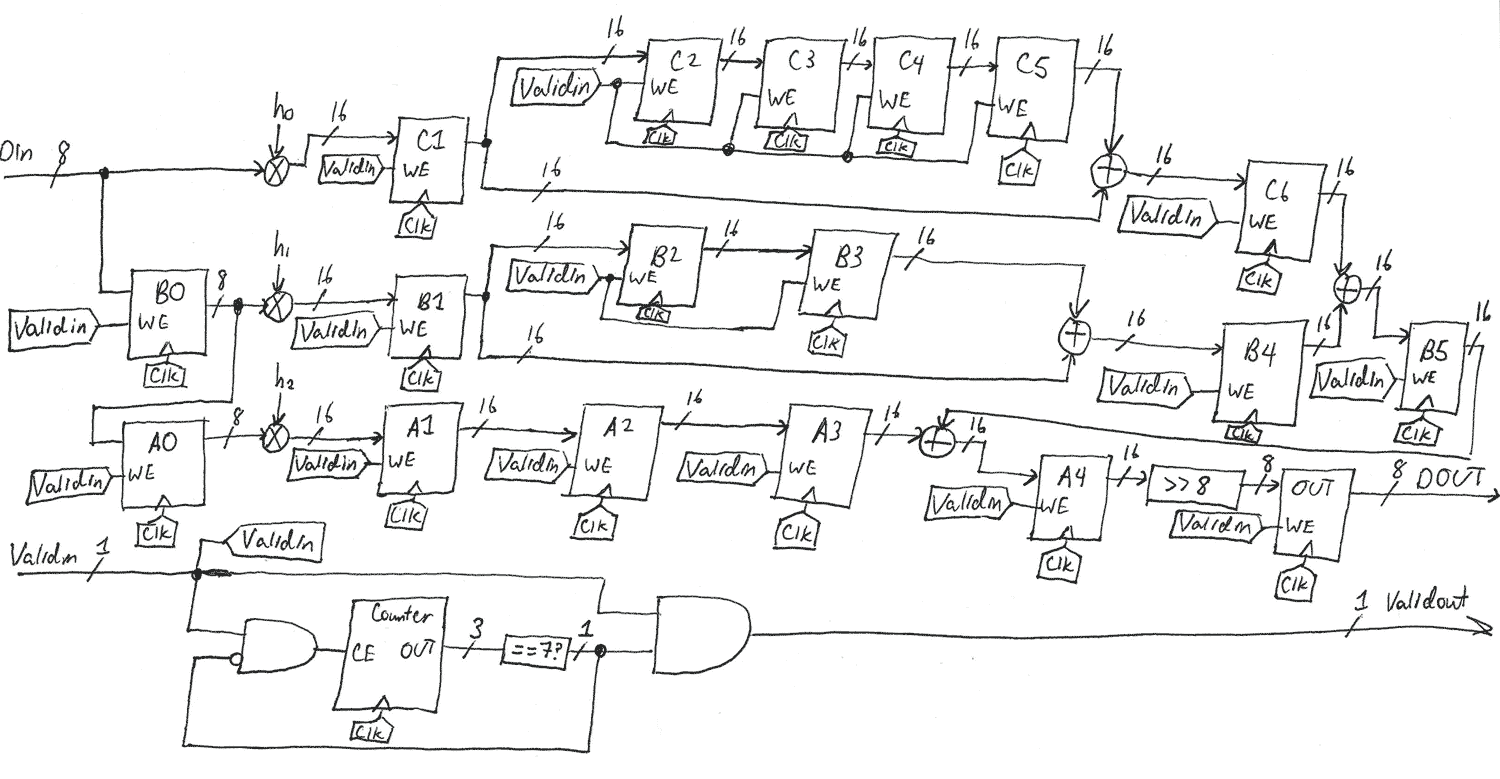
\includegraphics[scale=0.15]{modules/x_window.png}

Y Window Module:

\noindent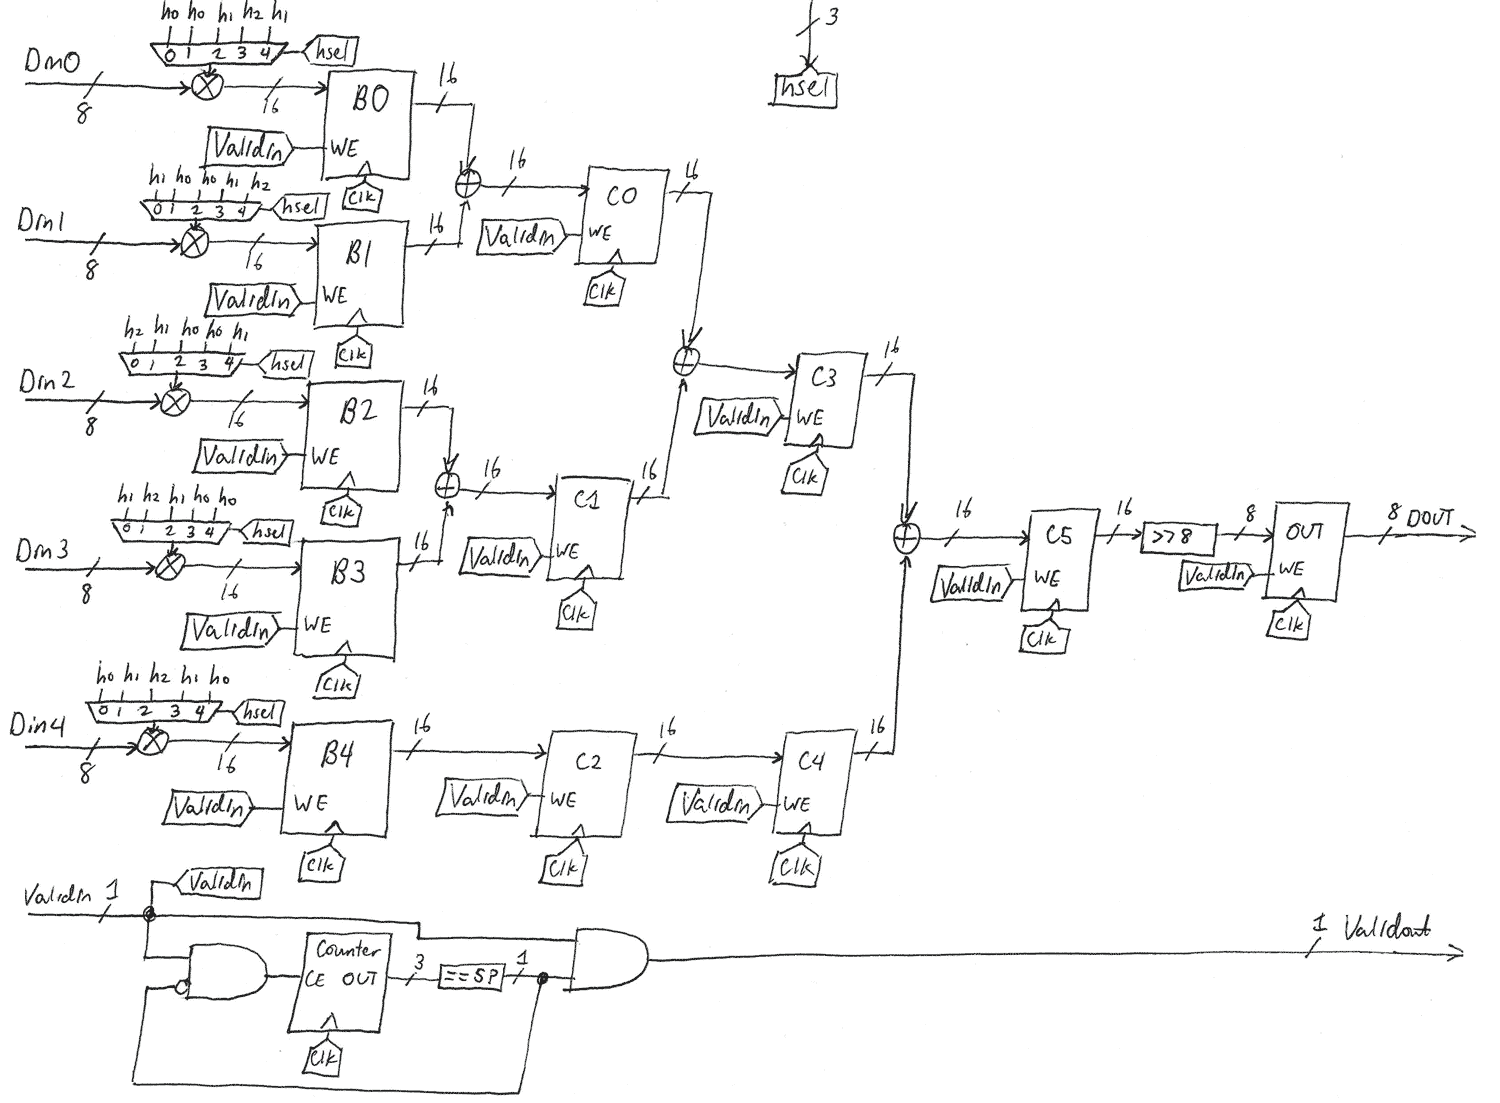
\includegraphics[scale=0.15]{modules/y_window.png}

5 Row Array Module:

Shift registers are 420 bytes wide.

\noindent\includegraphics[scale=0.15]{modules/5row.png}

\subsection*{b. Downsampling}

800x600 to 420x320 downsampler (2x + adds padding):

\noindent\includegraphics[scale=0.15]{modules/downsampler2x.png}

420x320 to 210x160 downsampler (2x)

\noindent\includegraphics[scale=0.15]{modules/downsampler2x_simple.png}

\subsection*{c. Upsampling}

Upsample 2x:

\noindent\includegraphics[scale=0.15]{modules/upsample2x.png}

Upsample 4x:

\noindent\includegraphics[scale=0.15]{modules/upsample4x.png}

\subsection*{d. Interface Connections}

(See overall diagram)

\section*{2. List of Signals}

\subsection*{Datapath Inputs}

\indent8 bit Data In (from VGA controller)

1 bit Valid  (from VGA controller)

1 bit DTACK (from VGA controller)

3 external clocks (not necessarily different clocks, but can be to reduce stalls)

1 bit out\_sel: selects which octave to output if orig/dog = dog

1 bit orig/dog: 0 indicates output VGA input, 1 indicates output dog octave indicated by out\_sel

5 bit ASEL into 5 Row Array Module

3 bit HSEL into Y Window Module

\subsection*{Datapath Outputs}

8 bit Data Out

1 bit Valid Out

18 bit Address Out (from Address Generator block)

1 bit output clock (for checkpoint 2 write clock)

\section*{3. RT Language Description}

\subsection*{Octave Module}
\begin{lstlisting}
while(true){
    Dog0ShiftReg <- (D1 << 2111*8) | (Dog0ShiftReg >> 8),
    Dog1ShiftReg <- (D2 << 2111*8) | (Dog1ShiftReg >> 8),
    Dog2ShiftReg <- (D3 << 2111*8) | (Dog2ShiftReg >> 8),
    Dog3ShiftReg <- (D4 << 2111*8) | (Dog3ShiftReg >> 8),
    Dog4ShiftReg <- (D5 << 2111*8) | (Dog4ShiftReg >> 8),
    Dog0Reg <- Dog0ShiftReg - D2,
    Dog1Reg <- Dog1ShiftReg - D3,
    Dog2Reg <- Dog2ShiftReg - D4,
    Dog3Reg <- Dog3ShiftReg - D5,
    Dog4Reg <- Dog4ShiftReg - D6,
    Valid0Reg <- V2,
    Valid1Reg <- V3,
    Valid2Reg <- V4,
    Valid3Reg <- V5,
    Valid4Reg <- V6;
}
\end{lstlisting}

\subsection*{5x5 Window Module}
\begin{lstlisting}
while(true){
    DelayShiftReg <- (BlankingRegion << 2111) | (DelayShiftReg >> 1),
    XWindow Ops, 5x5 Array Ops, YWindow Ops;
}
\end{lstlisting}

\subsection*{X Window Module}
\begin{lstlisting}

while(true){
    if(ValidIn) {
        B0 <- Din, A0 <- B0, C1 <- h0*Din, B1 <- h1*B0, 
        A1 <- h2*A0, C2 <- C1, C3 <- C2, C4 <- C3, 
        C5 <- C4, C6 <- C5 + C1, B2 <- B1, B3 <- B2, 
        B4 <- B3 + B1, B5 <- C6 + B4, A2 <- A1, 
        A3 <- A2, A4 <- B5 + A3, Out <- 1/5 * A4, 
        Counter <- Counter + 1 if Counter != 7;
    }
}
\end{lstlisting}

\subsection*{Y Window Module}
\begin{lstlisting}
while(true){
    if(ValidIn){
        B0 <- coeff*DIN0, 
        B1 <- coeff*DIN1, 
        B2 <- coeff*DIN2, 
        B3 <- coeff*DIN3, 
        B4 <- coeff*DIN4, 
        C0 <- B0 + B1, C1 <- B2 + B3, 
        C2 <- B4, C3 <- C0 + C1, C4 <- C2, 
        C5 <- C3 + C4, Out <- 1/5*C5, 
        Counter = Counter + 1 if Counter != 5;
    }
}
\end{lstlisting}

\subsection*{5 Row Array Module}

\begin{lstlisting}
while(true){
    if(ValidIn){
        ShiftReg0 <- {(DIN if ASEL[0] else (ShiftReg0 & 0xFF)),  (ShiftReg0 >> 8)},
        ShiftReg1 <- {(DIN if ASEL[1] else (ShiftReg1 & 0xFF)),  (ShiftReg1 >> 8)},
        ShiftReg2 <- {(DIN if ASEL[2] else (ShiftReg2 & 0xFF)),  (ShiftReg2 >> 8)},
        ShiftReg3 <- {(DIN if ASEL[3] else (ShiftReg3 & 0xFF)),  (ShiftReg3 >> 8)},
        ShiftReg4 <- {(DIN if ASEL[4] else (ShiftReg4 & 0xFF)),  (ShiftReg4 >> 8)},
        Counter = Counter + 1 if Counter != 3*WIDTH;
    }
}
\end{lstlisting}

\subsection*{2x Downsampler}
\begin{lstlisting}
while(true){
    DataoutReg <- 0x00 if PrevBlankingRegion else Data,
    RowCounter <- RowCounter + 1 if ColCounter == 839 else RowCounter,
    ColCounter <- ColCounter + 1 if valid & PrevBlankingRegion else ColCounter,
    ValidOutReg <- ColCounter % 2 == 0 && RowCounter % 2 == 0;
}
\end{lstlisting}

\subsection*{2x Downsampler Simple}
\begin{lstlisting}
while(true){
    DataoutReg <- Data,
    RowCounter <- RowCounter + 1 if ColCounter == 419 else RowCounter,
    ColCounter <- ColCounter + 1 if valid else ColCounter,
    ValidOutReg <- ColCounter % 2 == 0 && RowCounter % 2 == 0;
}
\end{lstlisting}

\subsection*{2x Upsample}
\begin{lstlisting}
while(true){
    DoutReg <- Dout, 
    PrevValid <- valid, ColCount <- ColCount + 1 if valid or PrevValid else ColCount, 
    RowCount <- RowCount + 1 if ColCount == 840 else RowCount, 
    ValidOutReg <- (PrevValid | Valid | (RowCount % 2 == 1)) & ColCount < 800 & RowCount < 600, 
    MuxSelReg <- RowCount % 2 == 1, 
    ShiftReg <- (ShiftReg >> 8) | (DoutReg << 839*8);
}
\end{lstlisting}

\subsection*{4x Upsample}
\begin{lstlisting}
while(true){
    DoutReg <- Dout, 
    PrevValid <- valid, 
    ColCount <- ColCount + 1 if valid or PrevValid else ColCount, 
    RowCount <- RowCount + 1 if ColCount == 840 else RowCount, 
    ValidOutReg <- (PrevValid | Valid | (RowCount % 4 != 0) | Prev-1Valid | Prev-2Valid) & ColCount < 800 & RowCount < 600, 
    MuxSelReg <- RowCount % 4 != 0, ShiftReg <- (ShiftReg >> 8) | (DoutReg << 839*8) if ShiftIn else (ShiftReg >> 8) | (ShiftReg << 839*8), 
    Prev-1Valid <- PrevValid, 
    Prev-2Valid <- Prev-1Valid;
}
\end{lstlisting}


\section*{4. Controller State Diagram}

\section*{5. Testbench Outline}

\end{document}
